\documentclass[11pt]{beamer}

%%%%%%%% tema e cor %%%%%%%%
\mode<presentation> {
\usetheme{Madrid}
%\usecolortheme{albatross}
}

\usepackage[utf8]{inputenc}
\usepackage{graphicx} 
\usepackage{booktabs}
\usepackage{subcaption}


\institute[HU-Berlin] 
{

\includegraphics[width=1.8cm]{img/logo-hu.png}
}

%%%%%%%% titulo e subtitulo %%%%%%%%
\title[Maximum Cardinality Matching]{Maximum Cardinality Matching Problem} 

%%%%%%%% nome dos autores %%%%%%%%
\author [Bojikian, Witkowski, Vogel]{Narek Bojikian, Piotr Witkowski, Martin Vogel} 

\begin{document}

\begin{frame}
\titlepage 
\end{frame}

%%%%%%%% slides %%%%%%%%
\section{Introduction} 
\begin{frame}{Assignment Problem}
\begin{figure}
    \centering
    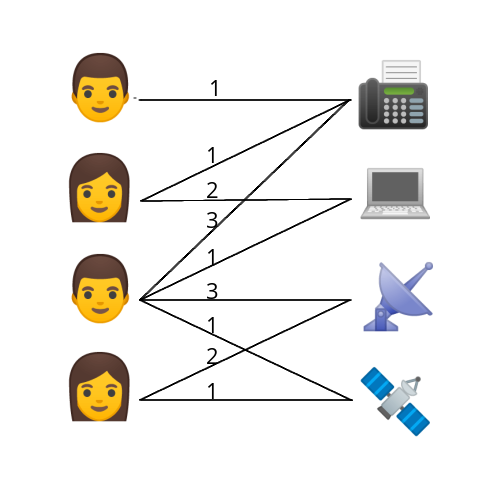
\includegraphics[height=5cm]{img/introduction/assignment.png}
\end{figure}
\end{frame}

\begin{frame}{Definitions}
        \begin{itemize}[<+->]
    \item Matching
    \item \textbf{Perfect} Matching
    \item \textbf{Bipartite} Matching
    \item \textbf{Maximum} Matching
    \end{itemize}
  
  %add different figure for perfect matching and bipartite matching  
\only<1>{
\begin{figure}
\begin{subfigure}{.5\textwidth}
\centering

\includegraphics[width=.4\linewidth]{img/introduction/graph01.eps}
\end{subfigure}%
\begin{subfigure}{.5\textwidth}
\centering
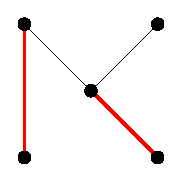
\includegraphics[width=.4\linewidth]{img/introduction/graph02.eps}
\end{subfigure}
\end{figure}
}
\only<2>
{
\begin{figure}
    \centering
    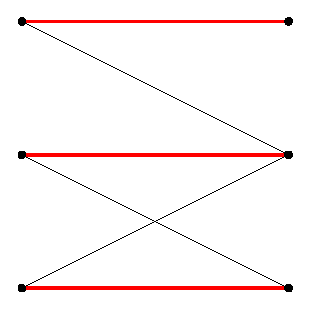
\includegraphics[width=0.3\linewidth]{img/introduction/perfectmatching.eps}
\end{figure}
}
\only<3>{
\begin{figure}
\begin{subfigure}{.5\textwidth}
\centering

\includegraphics[width=.4\linewidth]{img/introduction/bipar.eps}
\end{subfigure}%
\begin{subfigure}{.5\textwidth}
\centering
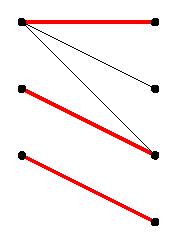
\includegraphics[width=.4\linewidth]{img/introduction/biparmatch.eps}
\end{subfigure}
\end{figure}
}
\only<4>{
\begin{figure}
\begin{subfigure}{.5\textwidth}
\centering
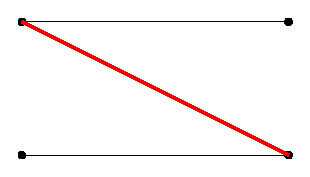
\includegraphics[width=.4\linewidth]{img/introduction/maximalmatch.eps}
\end{subfigure}%
\begin{subfigure}{.5\textwidth}
\centering

\includegraphics[width=.4\linewidth]{img/introduction/maximummatching.eps}
\end{subfigure}
\end{figure}
}
    
\begin{block}{Definition}
    \only<1>{A set of non overlapping edges.}
    \only<2>{Matching of size $\frac{|V\left(G\right)|}{2}$}
    \only<3>{Matching of the maximum size.}
    \only<4>{Matching on a bipartite graph.}
\end{block} 
\end{frame}


\section{Matching algorithms} 
\input{files/algos.tex}

\section{Approximation algorithms for matching} 
\input{files/approx.tex}

\section{Randomized Algorithm for matching} 
\begin{frame}{}
	\centering \textbf{\huge A short review..}
\end{frame}

\begin{frame}{Maximum Matching vs Maximal Matching}
	\parbox[c][.7\textheight][c]{\textwidth}{%
\only<1>
{
	\begin{center}
    
\includegraphics[width=0.15\linewidth]{img/random/maximum-maximal-0.eps}
	\end{center}
}
\only<2>
{
	\begin{center}
    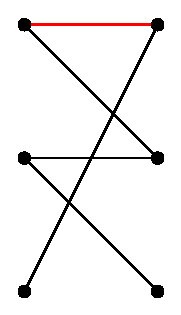
\includegraphics[width=0.15\linewidth]{img/random/maximum-maximal-1.eps}
	\end{center}
}
\only<3->
{
	\begin{center}
    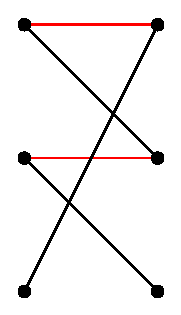
\includegraphics[width=0.15\linewidth]{img/random/maximum-maximal-2.eps}
	\end{center}
}
\uncover<4>
{
	\begin{center}
    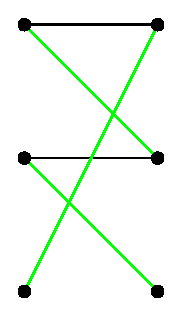
\includegraphics[width=0.15\linewidth]{img/random/maximum-maximal-3.eps}
	\end{center}
}
}
\end{frame}

\begin{frame}[t]{Determinant and Permanent}
	\uncover<2->{
	A short tour in number theory,\\
	}
	\uncover<3->{
		\textbf{Permutation} } \uncover<4->{ - Bijection over $n$ elements to them selves.}\\
	\only<5>{
\begin{tabular}{ |c|c|c|c|c|c| } 
 \hline
	$i$ & 1 & 2 & 3 & 4 & 5 \\ 
\hline
	$\delta (i)$ & 3 & 2 & 4 & 1 & 5\\ 
 \hline
\end{tabular}
		}

	\uncover<6->{	
	$\mathcal{S}_n$ - Set of all permutatoins of $n$ elements.\\~\\
	}
	\uncover<7->{
	For an $n\times n$-matrix $A$, we define
	}
\begin{columns}[T] % align columns\end{column}%
	\uncover<8->{
\begin{column}{.48\textwidth}
	{\centering \textbf{Determinant of a matrix}\\}
$$det(A) =  \sum\limits_{\pi \in \mathcal{S}} sign(\pi) \prod\limits_{i\in[n]} A_{i, \pi(i)}$$
	\uncover<10->{
	laplace expansion (on board).\\
	Efficient Gaussian Eliminatin.\\
	$O(n^\omega), \omega = 2.373$.\\
	Matrix-Multiplication Exponent.\\
	}

\end{column}
}
\hfill%
	\uncover<9->{
\begin{column}{.48\textwidth}
	{\centering \textbf{Permanent of a matrix}\\~\\}
$$perm(A) =  \sum\limits_{\pi \in \mathcal{S}}  \prod\limits_{i\in[n]} A_{i, \pi(i)}$$
	\uncover<11->{
	\textbf{NP-Hard} problem.\\
	Presumably no polynomial time algorithm to compute.\\
	}

\end{column}
}
\end{columns}
\end{frame}

\begin{frame}[t]{Randomized Perfect Matching}
	How to check if a bipartite graph admits a perfect matching?\\

\begin{tabular}{cl}  
\begin{tabular}{c}
\only<1-2>
{
    
\includegraphics[width=0.15\linewidth]{img/random/randombip-orig.eps}
}
\only<3->
{
    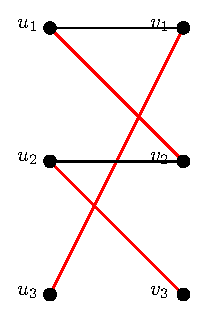
\includegraphics[width=0.15\linewidth]{img/random/randombip-matched.eps}
}
\end{tabular}
& \begin{tabular}{l}
\parbox{0.7\linewidth}{%  change the parbox width as appropiate
	\only<2-3>
	{
	\[
	A^G=
	\begin{bmatrix}
	1 & 1 & 0 \\
	0 & 1 & 1 \\
	1 & 0 & 0 
	\end{bmatrix}
	\]
	}
	\only<4->
	{
	\[
	A^G=
	\begin{bmatrix}
	1 & \textcolor{red}{1} & 0 \\
	0 & 1 & \textcolor{red}{1} \\
	\textcolor{red}{1} & 0 & 0 
	\end{bmatrix}
	\]
	}

\uncover<5->
{
	\begin{center}
	\begin{tabular}{|l|*{3}{c}|r}
		\hline
		$u_i$ & 1 &  2 & 3  \\
		\hline
		$\pi(u_i)$ & 2 &  3 & 1  \\
		\hline
	\end{tabular}
	\end{center}
}
}
\\
\end{tabular}
\end{tabular}
\only<6->
{
	The graph admits a perfect matching $\iff$\\
}
\only<7->
{
	There is a permutation $\pi$, s.t. $\prod\limits_{i \in [n]}A^G_{i, \pi(i)} = 1$  $\iff$\\
}
\only<8>
{
	For $\mathcal{S}$ the set of all permutations on $n$ elements
\[
	\sum\limits_{\pi \in \mathcal{S} } \prod\limits_{i \in [n]} A^G_{i, \pi(i)} > 0
\]
}
\only<9->
{
For $\mathcal{S}$ the set of all permutations on $n$ elements
\[
	\underbrace{\sum\limits_{\pi \in \mathcal{S} } \prod\limits_{i \in [n]} A^G_{i, \pi(i)}}_{perm(A^G)} > 0
\]
}
\end{frame}

\begin{frame}[t]{Permanent and Determinant}
	\begin{align*}
		perm(A) = & \sum\limits_{\pi \in \mathcal{S}} \prod\limits_{i\in[n]} A_{i, \pi(i)} & \uncover<2->{\dots\text{is a known hard problem}}\\
		\uncover<3->{det(A) = & \sum\limits_{\pi \in \mathcal{S}} sign(\pi) \prod\limits_{i\in[n]} A_{i, \pi(i)} & }
	\end{align*}

	\uncover<4->{We don't have to bound ourselves with ones in the matrix..\\}
	\uncover<5->{
	\begin{tabular}{cl}  
	\begin{tabular}{c}
    	
\includegraphics[width=0.15\linewidth]{img/random/randombip-orig.eps}
	\end{tabular}
	\begin{tabular}{l}
	\parbox{0.7\linewidth}{%  change the parbox width as appropiate
	\[
	A'^G=
	\begin{bmatrix}
		x_{11} & x_{12} & 0 \\
		0 & x_{22} & x_{23} \\
		x_{31} & 0 & 0 
	\end{bmatrix}
	\]
	}
	\end{tabular}
	\end{tabular}
	}
	\uncover<6->{$det(A'^G)$ is a polynomial of degree $n$.\\}
	\uncover<7->{The graph admits a perfect matching $\iff$ the polynomial $det(A'^G)$ is not identical zero.}
\end{frame}

\begin{frame}[t]{Schwartz-Zippel lemma} 
	\begin{block}{Shwartz-Zippel lemma}
		Let $\rho$ be a non-zero polynomial of $n$ variables and degree $d$ over a field $\mathbb{F}$.\\
		Let $\mathcal{S} \subseteq \mathbb{F}^n$, then for $x_0 \underset{u.a.r}{\in} \mathcal{S}$
		$$Pr[\rho(x_0) = 0] \leq \frac{d}{|\mathcal{S}|}$$
	\end{block}
	\only<2->
	{
	Choosing $|\mathcal{S}| = 2d$, we get a method that tells with probability at least $1/2$, if the polynomial is identical zero.\\
	}
	\only<3->
	{
	Since one non-zero answer is enough to know the polynomial is a non-zero, we can repeat the operation a couple of times magnifying the probability.\\
	}
\end{frame}



\section{Conclusion} 
\input{files/conclusion.tex}
\end{document}
